% Lab03: Mineração de Métricas DORA. Compila no template da SBC do Overleaf (ver README do lab03).
\documentclass[12pt]{article}

\usepackage{sbc-template}
\usepackage{graphicx,url}
\usepackage[utf8]{inputenc}
\usepackage[brazil]{babel}
\usepackage{amsmath}

\sloppy

\title{Métricas DORA em repositórios populares do GitHub:\\
o que dá para medir só com dados públicos}

\author{Athos Marques Ribeiro Fonseca\inst{1}, Mateus Araujo Santos\inst{1},\\
Rafael Ganascini de Moura\inst{1}}

\address{Pontifícia Universidade Católica de Minas Gerais (PUC Minas)\\
Curso de Engenharia de Software\\
Laboratório de Experimentação de Software (Prof. Danilo Maia)}

\begin{document}

\maketitle

\begin{abstract}
DORA metrics are the usual way to describe how fast and how safely a team delivers software, but
open-source projects on GitHub do not record deployments or incidents. We measured the four metrics
in 310 popular repositories that use GitHub Actions, replacing deployments with published releases
and incidents with failed CI runs and corrective releases. The typical repository publishes 0.46
releases per week, has a median lead time of 354 hours, a CI failure rate of 4.7\% and recovers from
a red build in 2.9 hours; 43\% are classified as Medium. The classification is unstable: between 32\%
and 43\% of the repositories change category when the operational definition changes (weighted
kappa from 0.39 to 0.52), and the choice of change failure rate weighs much more than the deployment
unit. Repositories with commits made by coding agents publish slightly more often, but the intensity
of use is not associated with any metric.
\end{abstract}

\begin{resumo}
As métricas DORA são a forma mais usada de descrever o quão rápido e com quanta segurança um time
entrega software, mas projetos open-source no GitHub não registram deploys nem incidentes. Medimos
as quatro métricas em 310 repositórios populares que usam GitHub Actions, trocando deploy por release
publicada e incidente por execução de CI com falha e por release corretiva. O repositório típico
publica 0,46 release por semana, tem \textit{lead time} mediano de 354 horas, 4,7\% de falhas no CI e
se recupera de um build vermelho em 2,9 horas; 43\% ficam em \textit{Medium}. A classificação é
instável: entre 32\% e 43\% dos repositórios mudam de categoria quando a definição operacional muda
(kappa ponderado de 0,39 a 0,52), e a escolha da taxa de falha pesa bem mais que a unidade de deploy.
Repositórios com commits feitos por agentes de programação publicam um pouco mais, mas a intensidade
de uso não se associa a nenhuma métrica.
\end{resumo}

\section{Introdução}

O DORA (\textit{DevOps Research and Assessment}) propôs quatro métricas de entrega de software:
frequência de deploy, \textit{lead time} das mudanças, taxa de falha das mudanças (\textit{change
failure rate}, CFR) e tempo de recuperação \cite{forsgren2018accelerate,dora2024}. As duas primeiras
medem velocidade e as duas últimas, estabilidade, e a afirmação mais conhecida do DORA é que as duas
não competem entre si. Esses números vêm de questionários sobre sistemas com deploy em produção e
incidentes registrados. Um repositório open-source no GitHub não tem nenhum dos dois, só dados
parecidos: releases publicadas, commits com data e execuções de CI. Cada troca tem um buraco
conhecido. A release de uma biblioteca não coloca nada em produção, um CI vermelho pode ser um teste
instável e uma release corretiva pode ser só uma dependência atualizada às pressas. Por isso o
resultado depende da definição escolhida.

Medimos as quatro métricas em 310 repositórios populares que usam GitHub Actions, numa janela de 12
meses, só com dados públicos da API do GitHub, com duas variantes de \textit{lead time} e de CFR.
As hipóteses abaixo foram escritas antes da coleta da amostra, por quem implementou a parte do
pipeline ligada a cada questão; até então só tínhamos visto os três repositórios de teste do
pipeline, que não entram na análise.

\begin{itemize}
\item \textbf{RQ 01. Qual a frequência de deploys?} Mediana entre \textit{Medium} e \textit{High}
(uma release por mês a sete por semana), mais perto do limite inferior, porque bibliotecas agrupam
mudanças antes de publicar, com distribuição assimétrica e poucos repositórios em \textit{Elite}.
\item \textbf{RQ 02. Qual o tempo entre um commit e seu deploy?} A variante por release (a) maior
que a por commit (b) em mais de 90\% dos repositórios, com mediana da (a) entre 2 e 4 semanas e cerca
de um terço em \textit{Low}; a (b) entre 40\% e 60\% da (a); categoria mudando entre as variantes em
cerca de metade dos repositórios.
\item \textbf{RQ 03. Qual a taxa de falha das mudanças?} CFR de CI (a) em \textit{Elite}
($\leq$ 15\%), porque quase tudo passa pelo CI do PR antes do \texttt{main}; CFR de entrega (b) em
\textit{High} (15\% a 30\%), porque a \texttt{x.y.1} logo depois da \texttt{x.y.0} é comum; pouca
concordância entre as duas.
\item \textbf{RQ 04. Qual o tempo de recuperação após uma falha de CI?} Mediana em \textit{High}
(1 hora a 1 dia), já que CI vermelho no \texttt{main} trava todo mundo, com IQR largo e episódios
censurados concentrados em workflows secundários.
\item \textbf{RQ 05. Mais deploys vêm com mais ou menos falhas?} Correlação fraca com a CFR (a)
($|\rho| < 0{,}2$) e positiva e moderada com a CFR (b) ($0{,}3$ a $0{,}5$), esta última em boa
parte artefato da medida: quem solta release toda semana quase sempre tem outra em até 7 dias.
\item \textbf{RQ 06. Que características acompanham um desempenho melhor?} Repositórios mais
populares, antigos e com mais contribuidores melhores, sobretudo em frequência e \textit{lead time},
com efeitos pequenos ou moderados e diferentes por métrica.
\item \textbf{RQ 07. O quanto a classificação depende da definição?} De 30\% a 50\% dos
repositórios mudando de categoria, kappa ponderado entre 0,40 e 0,60, com a unidade de deploy (tag
no lugar de release) como a escolha que mais pesa e trocas quase sempre para a categoria vizinha.
\item \textbf{RQ 08 (bônus). Como a \textit{rework rate} se compara à CFR (b)?} Sem hipótese prévia.
\item \textbf{RQ 09 (extra). Adotar agentes de programação muda o desempenho DORA?} Escrita depois
de vermos as métricas, mas antes de cruzá-las com a adoção: \textit{lead time} igual ou menor e CFR
(a) maior nos adotantes, já que o DORA 2024 associou IA a lotes maiores e menos estabilidade
\cite{dora2024} e os commits com agente são maiores \cite{robbes2026agentic}, mas sem diferença grande,
porque quem usa IA sem deixar rastro fica entre os não adotantes.
\end{itemize}

\section{Metodologia}

\paragraph{Fonte de dados e seleção.} Os dados vêm da API REST do GitHub, por um pipeline próprio
com cache em disco e espera automática no limite de requisições. A janela vai de 1º de outubro de
2025 a 30 de setembro de 2026 (UTC). Os candidatos são os 60.188 repositórios com pelo menos mil
estrelas, sem \textit{fork} nem arquivados, avaliados do mais estrelado para baixo. Para passar do
teto de mil resultados da busca, cada consulta pede as estrelas abaixo do menor valor visto na
anterior. Cada candidato precisa ter sido criado antes da janela, usar GitHub Actions, ter pelo menos
5 releases e pelo menos 50 execuções válidas de CI por \textit{push} no branch principal dentro da
janela. A avaliação parou quando 310 passaram (Tabela~\ref{tab:funil}), e só então foram coletados os
commits de cada release e todas as execuções de CI. O filtro que mais pesa é o de releases. Como a
avaliação para em 310, a amostra fica entre 37 mil e 254 mil estrelas. No total são 22.609 releases e
3.167.550 execuções válidas de CI.

\begin{table}[ht]
\centering
\caption{Funil de seleção da amostra}
\label{tab:funil}
\small
\begin{tabular}{lrr}
\hline
Etapa & Restantes & Descartados \\
\hline
Avaliados, do mais estrelado para baixo (de 60.188) & 845 & \\
Criados antes do início da janela & 761 & 84 \\
Com GitHub Actions & 685 & 76 \\
$\geq$ 5 releases na janela & 362 & 323 \\
$\geq$ 50 execuções válidas na janela (amostra final) & 310 & 52 \\
\hline
\end{tabular}
\end{table}

\paragraph{Definições operacionais.} Deploy é uma release publicada que não é pré-release. Só entra o
branch padrão. O \textit{lead time} (a) é a mediana, por release, entre a publicação e o commit mais
antigo do \texttt{compare} com a release estável anterior, e o (b) é a mediana de todos os pares
commit--release, com a data de autor do commit. No CI entram só execuções por \textit{push}: contam
\texttt{success}, \texttt{failure}, \texttt{timed\_out} e \texttt{startup\_failure}, e as demais
conclusões são ignoradas. A CFR (a) é a fração de execuções com falha. Na CFR (b), uma release falha
quando a seguinte sai em até 7 dias e é corretiva; releases dos últimos 7 dias da janela são
censuradas. Um episódio de recuperação vai da primeira falha de um workflow depois de um sucesso até o
sucesso seguinte; episódios sem sucesso posterior são censurados e ficam fora da mediana. A
classificação geral (C1) é a mediana das faixas de frequência, \textit{lead time} (a) e CFR (a),
arredondada para baixo. O enunciado usa as quatro métricas, mas deixamos a recuperação de fora: ela
vem só do CI e não muda entre as combinações da RQ 07, e, como fica em \textit{High} em 70\% da
amostra, puxaria a nota de todos para o meio e esconderia as diferenças entre as definições. Com as
quatro métricas, 68 repositórios (22\%) mudariam de categoria, 56 deles para cima (os \textit{Low}
cairiam de 55 para 19). A RQ 07 troca a unidade de deploy: na C2 as pré-releases também contam, e na
C3 a unidade é a tag com \texttt{X.Y} ou \texttt{X.Y.Z} no nome, datada pelo commit apontado (sem esse
filtro entrariam milhares de tags criadas pelo CI, como no \texttt{pytorch/pytorch}).

\paragraph{Heurística de release corretiva.} Uma release é corretiva quando o objetivo principal
dela é corrigir um defeito recente. Testamos quatro regras contra o consenso dos três avaliadores
(Tabela~\ref{tab:heuristica}). A v1, sugerida no enunciado, marca 278 das 300 releases, porque quase
toda release tem algum commit com \texttt{fix}. A v2 perde recall nos repositórios com mais de uma
linha de versão, em que a release anterior pela data é de outra linha. A v4 é a usada na CFR (b).
Como as regras foram ajustadas olhando os erros nas mesmas 300 releases, o F1 tende a ser otimista.

\begin{table}[ht]
\centering
\caption{Versões da heurística de release corretiva contra o consenso (300 releases, 115 corretivas)}
\label{tab:heuristica}
\small
\begin{tabular}{lp{8.2cm}rrr}
\hline
Versão & Regra & Precisão & Recall & F1 \\
\hline
v1 & Só o \textit{patch} subiu \textbf{ou} algum commit tem \texttt{fix}, \texttt{hotfix} ou
\texttt{revert} & 0,399 & 0,965 & 0,565 \\
v2 & Só o \textit{patch} subiu \textbf{e} algum commit tem essas palavras & 0,541 & 0,626 & 0,581 \\
v3 & O \textit{patch} da própria versão é maior que zero & 0,542 & 0,904 & 0,678 \\
v4 & v3 \textbf{e} as notas citam correção pelo menos tantas vezes quanto novidade & 0,673 & 0,861
& 0,756 \\
\hline
\end{tabular}
\end{table}

\paragraph{Validação manual.} A amostra-ouro tem 60 repositórios sorteados da amostra final e 5
releases de cada um (300 releases), com semente fixa (\texttt{random\_state=42}). Cada integrante
rotulou sozinho, sem ver os outros nem a saída da heurística, o tipo do projeto, se as releases chegam
a quem usa o projeto e se cada release é corretiva. A concordância é medida pelo kappa de Fleiss com a
interpretação de Landis e Koch, e o consenso é por maioria; não houve nenhum caso de três rótulos
diferentes. A Tabela~\ref{tab:kappa} mostra a concordância. Nas entregas reais, o kappa moderado
convive com 98\% de concordância porque quase todos os rótulos são ``sim'' (59 dos 60 no consenso), e
o kappa cai mesmo com pouca discordância. A corretiva é a dimensão mais difícil: 72\% de concordância
simples, e o consenso marcou 115 das 300 releases. O sorteio expôs um problema que afeta o \textit{lead time}: em 9 das 300 releases a anterior
pela data tem versão maior (a \texttt{v8.19.14} do \texttt{elastic/elasticsearch} sai depois da
\texttt{v9.2.8}, e o \texttt{compare} entre elas tem 5.188 commits).

\begin{table}[ht]
\centering
\caption{Concordância entre os três avaliadores na amostra-ouro}
\label{tab:kappa}
\small
\begin{tabular}{lrrrl}
\hline
Dimensão & Itens & Concordância & $\kappa$ de Fleiss & Landis e Koch \\
\hline
Tipo do projeto & 60 & 91,7\% & 0,91 & quase perfeita \\
Entregas reais & 60 & 98,3\% & 0,49 & moderada \\
Release corretiva & 300 & 72,3\% & 0,61 & substancial \\
\hline
\end{tabular}
\end{table}

\paragraph{Análise.} As RQ 01 a 04 usam mediana e IQR, porque as distribuições são assimétricas.
A RQ 05 usa Spearman. A RQ 06 compara as métricas entre quartis de estrelas, contribuidores e idade
e entre as sete linguagens com pelo menos 10 repositórios (as demais viram ``Outras''), com
Kruskal-Wallis, $\varepsilon^2 = H/(n-1)$, correção de Holm nos 16 testes e delta de Cliff entre os
grupos dos extremos. A RQ 07 usa o kappa de Cohen com peso linear.

\paragraph{Detecção de agentes (RQ 09).} Um commit é feito com agente quando deixa rastro
explícito, nas famílias de Robbes et al. \cite{robbes2026agentic}: coautoria ou autoria do agente,
PR aberto de um branch do agente (\texttt{copilot/}, \texttt{codex/}, \texttt{claude/} etc.) ou label
do agente; o arquivo de instruções do agente marca o repositório. Foram 119.208 commits marcados. Num
sorteio de 100, os três avaliadores confirmaram os 100 pelo consenso (precisão de 100\%, de 89,7\% a
100\% por avaliador); o recall não foi medido. A adoção é a proporção de commits com agente desde o
primeiro, nos níveis de Robbes et al. (C1) e em três alternativas: tercis (C2) e quartis (C3) entre os
adotantes e versionar ou não o arquivo de instruções (C4). Essas regras foram commitadas antes de
qualquer cruzamento com as métricas. A comparação de antes e depois exige 91 dias sem rastro antes da
adoção e 91 depois.

\paragraph{Contribuições além do enunciado.} O que o grupo acrescentou por conta própria:
\begin{itemize}
\item \textbf{RQ 09}, uma questão nova sobre agentes de programação, com detecção validada à mão,
quatro classificações de adoção e três análises (entre repositórios, antes e depois da adoção e
commits com e sem agente no mesmo repositório).
\item \textbf{Notas da release na heurística corretiva (v4).} O enunciado sugere olhar a versão e as
mensagens de commit; somar as notas da release levou o F1 de 0,565 (v1) para 0,756.
\item \textbf{Uma escolha de cada vez na RQ 07.} Além dos pares de combinações pedidos, mudamos uma
definição por vez, o que mostrou que a CFR pesa mais que a unidade de deploy.
\item \textbf{Os cinco fatores na RQ 06} (o mínimo era três), com delta de Cliff entre os grupos dos
extremos para mostrar a direção de cada efeito.
\end{itemize}

\section{Resultados}

\paragraph{RQ 01 a 04.} A Tabela~\ref{tab:rq01-04} resume as métricas e a
Figura~\ref{fig:c1}, as faixas DORA. O repositório típico solta 0,46 release por semana (cerca de 24
por ano), e metade fica em \textit{Medium}. O \textit{lead time} mediano é de 354 horas na (a) e 400
na (b). A (a) é maior que a (b) em 186 de 309 repositórios (60,2\%), com mediana das razões de 1,28.
A CFR (a) põe 83,5\% da amostra em \textit{Elite}, e a (b) tem mediana de 25\%, em \textit{High}, com
59 repositórios (19,1\%) em zero. A recuperação mediana é de 2,91 horas; a mediana da proporção de
episódios censurados é zero e o terceiro quartil, 0,4\%; 16 repositórios não tiveram episódio.

\begin{table}[ht]
\centering
\caption{RQ 01 a 04: resumo das métricas e repositórios por faixa DORA}
\label{tab:rq01-04}
\small
\begin{tabular}{lrrrrrrrrr}
\hline
Métrica & $n$ & Mediana & Q1 & Q3 & IQR & Elite & High & Med. & Low \\
\hline
Releases/semana & 310 & 0,46 & 0,23 & 1,00 & 0,77 & 8 & 71 & 157 & 74 \\
\textit{Lead time} (a), h & 309 & 354 & 135 & 1.058 & 923 & 23 & 74 & 106 & 106 \\
\textit{Lead time} (b), h & 309 & 400 & 137 & 1.596 & 1.458 & 24 & 67 & 103 & 115 \\
CFR (a), \% & 310 & 4,7 & 2,3 & 11,1 & 8,8 & 259 & 34 & 10 & 7 \\
CFR (b), \% & 309 & 25,0 & 8,4 & 43,8 & 35,4 & 113 & 74 & 48 & 74 \\
Recuperação, h & 294 & 2,91 & 1,25 & 6,78 & 5,53 & 61 & 207 & 24 & 2 \\
\hline
Classificação C1 & 310 & & & & & 21 & 101 & 133 & 55 \\
\hline
\end{tabular}
\end{table}

\begin{figure}[ht]
\centering
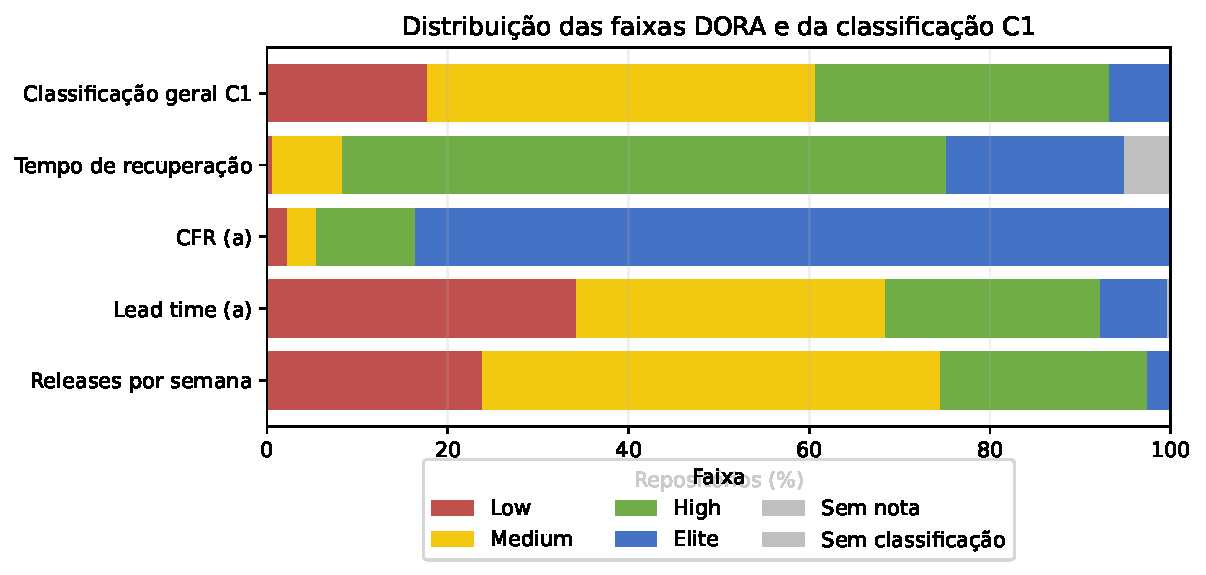
\includegraphics[width=0.75\textwidth]{figuras/classificacao_c1.pdf}
\caption{Faixas DORA das quatro métricas e da classificação geral C1}
\label{fig:c1}
\end{figure}

\paragraph{Classificação de referência (C1).} A C1 ficou com 6,8\% em \textit{Elite}, 32,6\% em
\textit{High}, 42,9\% em \textit{Medium} e 17,7\% em \textit{Low}. Frequência e \textit{lead time}
acompanham a categoria geral: 53 dos 55 \textit{Low} têm frequência \textit{Low} e os 55 têm
\textit{lead time} \textit{Low}. A CFR (a) é \textit{Elite} em 47 dos 55 \textit{Low}, então ela quase
nunca decide a categoria. Um repositório, sem \textit{lead time} (a), foi classificado com duas notas.

\paragraph{RQ 05.} As duas correlações com a frequência são positivas e significativas, mas de força
muito diferente: $\rho = 0{,}19$ com a CFR (a) ($n = 310$, $p < 0{,}001$) e $\rho = 0{,}62$ com a CFR
(b) ($n = 309$, $p < 0{,}001$). Os 59 repositórios com CFR (b) igual a zero soltam poucas releases
(mediana de 0,19 por semana, contra 0,56 nos demais) e formam a faixa de pontos no zero da
Figura~\ref{fig:rq05}; sem eles, o $\rho$ da (b) cai para 0,49 ($n = 250$, $p < 0{,}001$).

\begin{figure}[ht]
\centering
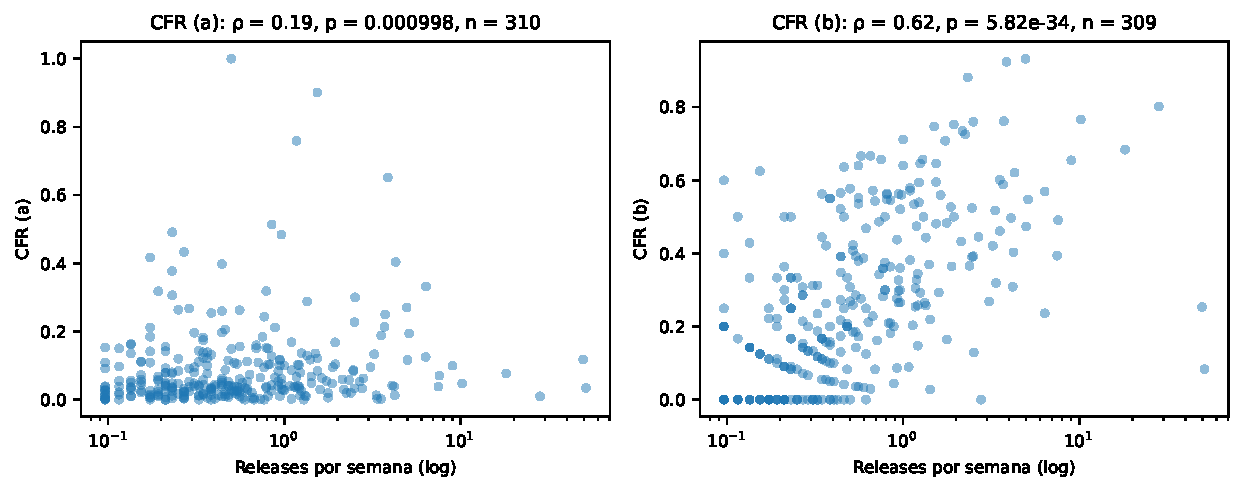
\includegraphics[width=0.9\textwidth]{figuras/rq05_dispersao.pdf}
\caption{RQ 05: releases por semana × CFR, um painel por variante. Eixo x em escala log}
\label{fig:rq05}
\end{figure}

\paragraph{RQ 06.} Das 16 combinações de fator e métrica, 4 continuam significativas depois do Holm
(Tabela~\ref{tab:rq06}): \textit{lead time} (a) por idade, por contribuidores e por linguagem, e
frequência por idade. Releases por linguagem fica no limite ($p$ ajustado de 0,0505). Nenhum fator
afeta a CFR (a) nem a recuperação, e as estrelas não afetam nada. O efeito mais forte é o da idade no
\textit{lead time} (a): a mediana sobe de 131 horas no 1º quartil para 293, 485 e 1.058 no 4º
($\delta = 0{,}70$, grande). Os mais novos também soltam mais releases (0,85 contra 0,35 por semana,
$\delta = -0{,}44$). Nos contribuidores, o efeito está quase todo no 4º quartil (1.024 horas,
$\delta = 0{,}52$), e entre as linguagens C++ tem a maior mediana (2.157 horas, $n = 16$) e TypeScript
a menor (241 horas, $\delta = 0{,}59$). Na amostra-ouro, o tipo de projeto não muda nenhuma métrica
($p$ entre 0,43 e 0,64).

\begin{table}[ht]
\centering
\caption{RQ 06: Kruskal-Wallis, $p$ ajustado por Holm (16 testes) e $\varepsilon^2$}
\label{tab:rq06}
\small
\begin{tabular}{lrrrrrrrr}
\hline
& \multicolumn{2}{c}{Releases/sem.} & \multicolumn{2}{c}{\textit{Lead time} (a)} &
\multicolumn{2}{c}{CFR (a)} & \multicolumn{2}{c}{Recuperação} \\
Fator & $p$ aj. & $\varepsilon^2$ & $p$ aj. & $\varepsilon^2$ & $p$ aj. & $\varepsilon^2$ & $p$ aj. &
$\varepsilon^2$ \\
\hline
Estrelas & 0,441 & 0,026 & 1,000 & 0,004 & 1,000 & 0,008 & 1,000 & 0,014 \\
Contribuidores & 0,175 & 0,033 & $<$0,001 & 0,114 & 0,843 & 0,016 & 1,000 & 0,013 \\
Idade & $<$0,001 & 0,080 & $<$0,001 & 0,232 & 0,532 & 0,021 & 0,441 & 0,028 \\
Linguagem & 0,0505 & 0,067 & $<$0,001 & 0,108 & 0,441 & 0,046 & 0,478 & 0,045 \\
\hline
\end{tabular}
\end{table}

\paragraph{RQ 07.} Entre 32\% e 43\% dos repositórios mudam de categoria geral em cada par de
combinações, e 166 dos 309 classificados nas três (53,7\%) mudam em pelo menos um
(Tabela~\ref{tab:rq07}). A C3 sobe a categoria de 89 repositórios e desce a de 31; a C2 desce 72 e
sobe 60. Quase todas as mudanças são para a categoria vizinha (80\% de C1 para C2 e 92\% de C1 para
C3), e saltos de três categorias aconteceram uma vez em cada par (Figura~\ref{fig:rq07}). Mudando uma escolha de cada vez, a
que mais pesa é a CFR: trocar a (a) pela (b) muda a faixa de 67\% dos repositórios, quase sempre para
pior (182 contra 26), com kappa zero. Trocar release por tag muda a frequência de 23\% e incluir
pré-releases, de 12\%.

\begin{table}[ht]
\centering
\caption{RQ 07: repositórios que mudam de faixa, por par de combinações e por escolha isolada}
\label{tab:rq07}
\small
\begin{tabular}{llrrr}
\hline
Comparação & Faixa comparada & $n$ & \% mudou & $\kappa$ \\
\hline
C1 × C2 & geral & 309 & 42,7 & 0,39 \\
C1 × C3 & geral & 310 & 38,7 & 0,52 \\
C2 × C3 & geral & 309 & 32,0 & 0,51 \\
\hline
CFR (a) × (b) & CFR & 309 & 67,3 & 0,00 \\
\textit{Lead time} (a) × (b) & \textit{lead time} & 309 & 41,7 & 0,54 \\
Release × tag & frequência & 310 & 22,6 & 0,67 \\
Release × release + pré-release & frequência & 310 & 11,6 & 0,85 \\
\hline
\end{tabular}
\end{table}

\begin{figure}[ht]
\centering
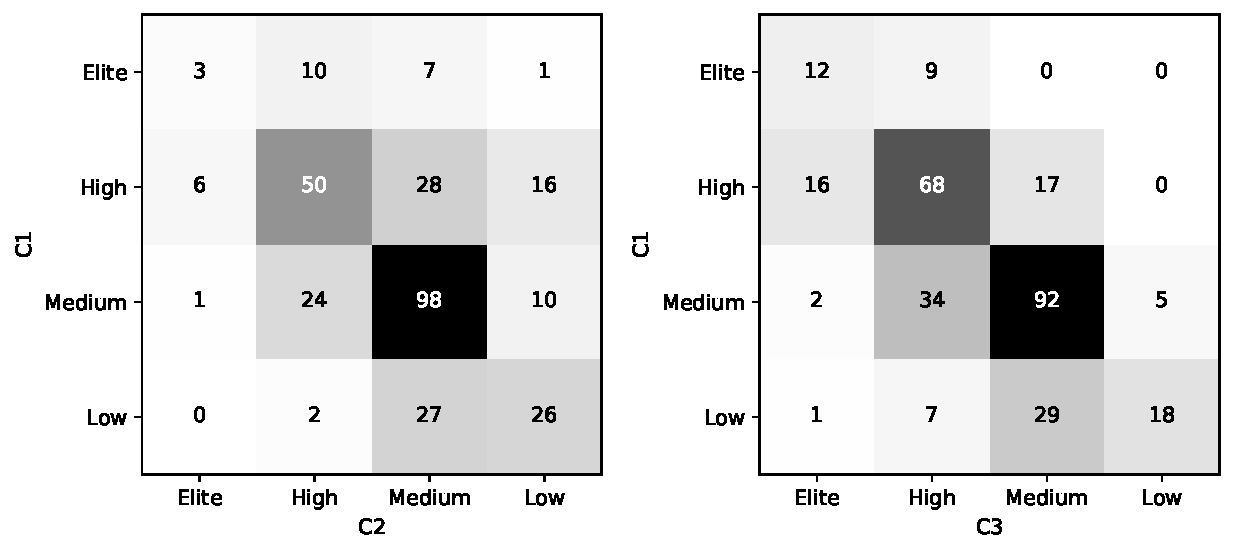
\includegraphics[width=0.7\textwidth]{figuras/rq07_transicoes.pdf}
\caption{RQ 07: transição de categoria geral de C1 para C2 e de C1 para C3 (contagem de repositórios)}
\label{fig:rq07}
\end{figure}

\paragraph{RQ 08.} A \textit{rework rate}, proporção de releases corretivas entre as que têm uma
anterior, tem mediana de 0,50 (IQR de 0,32 a 0,74). Ela se associa moderadamente à CFR (b)
($\rho = 0{,}54$, $p < 0{,}001$, $n = 309$) e é maior que ela em 267 repositórios. Os casos extremos,
como \texttt{pingcap/tidb}, \texttt{microsoft/terminal} e \texttt{qbittorrent/qBittorrent}, têm
\textit{rework rate} 1 e CFR (b) zero: todas as releases são corretivas, mas nenhuma sai até 7 dias
depois da anterior.

\paragraph{RQ 09.} Dos 310 repositórios, 282 têm pelo menos um commit com agente e 28 não têm
nenhum. Entre repositórios, a proporção de commits com agente se correlaciona fracamente com a
frequência ($\rho = 0{,}16$, $p$ ajustado de 0,022) e com o \textit{lead time} (a) ($\rho = -0{,}15$,
$p = 0{,}032$), mas as correlações somem entre os adotantes. Por nível, só a frequência difere: 0,22
release por semana sem adoção, 0,46 na adoção baixa e 0,50 na alta ($\varepsilon^2 = 0{,}03$). Quem
versiona o arquivo do agente (C4) solta mais releases (0,58 contra 0,31), tem \textit{lead time} menor
(272 contra 480 horas) e CFR (a) maior (5,6\% contra 3,5\%). Sem os 48 projetos que são eles mesmos
agentes ou assistentes de LLM, a correlação com a frequência some ($\rho = 0{,}11$, $p = 0{,}21$). Nos
105 adotantes com 91 dias de cada lado, nada muda entre antes e depois (Wilcoxon pareado). Dentro do
mesmo repositório, o commit com agente não demora mais para sair numa release (221 contra 196 horas,
$p = 0{,}62$), e a menor falha de CI dele (12,9\% contra 15,1\%) não sobrevive ao Holm.

\section{Discussão}

A Tabela~\ref{tab:hipoteses} confronta cada hipótese com o resultado.

\begin{table}[ht]
\centering
\caption{Hipóteses da Introdução e o resultado}
\label{tab:hipoteses}
\small
\begin{tabular}{lp{0.13\textwidth}p{0.68\textwidth}}
\hline
RQ & Confirmou? & O que os dados mostraram \\
\hline
01 & Em parte & Metade em \textit{Medium}, mas 23,9\% em \textit{Low} \\
02 & Em parte & Mediana da (a) e um terço em \textit{Low} como previsto, mas (a) $>$ (b) só em 60,2\% \\
03 & Sim & CFR (a) em \textit{Elite}, CFR (b) em \textit{High} e kappa zero entre elas \\
04 & Sim & Mediana de 2,91 horas, em \textit{High}; a cauda não foi verificada \\
05 & Em parte & Respostas diferentes, mas $\rho$ positivo na (a) e acima do previsto na (b) \\
06 & Em parte & Associações parciais, mas idade e contribuidores pioram o desempenho \\
07 & Em parte & Instabilidade do tamanho previsto, causada pela CFR e não pela unidade de deploy \\
09 & Não & Nenhum efeito da intensidade de uso; só ter ou não rastro de agente \\
\hline
\end{tabular}
\end{table}

\paragraph{O peso da definição de CFR.} A maior surpresa foi a CFR, e não a unidade de deploy,
dominar a instabilidade da classificação (RQ 07). As duas variantes medem coisas que quase não se
tocam: CI vermelho no \texttt{main} é raro, e correção logo depois de uma release é comum. Isso
também explica a RQ 05. O $\rho$ de 0,62 da CFR (b) pareceria um \textit{trade-off} entre velocidade e
estabilidade, contrário ao DORA, mas a medida mistura as duas coisas: uma release só falha se outra
sair em até 7 dias, o que é quase certo para quem solta várias por semana, e a própria release
corretiva conta como deploy. Por isso não lemos o resultado como ``ir rápido quebra mais''. A
\textit{rework rate} (RQ 08) mostra o mesmo de outro ângulo: sem o prazo de 7 dias, projetos de ciclo
longo com quase tudo corretivo têm CFR (b) zero. Com a CFR (a), a associação é fraca demais para
confirmar ou contradizer o DORA. Para as RQ 01 a 06, isso quer dizer que as tendências gerais se
sustentam, porque quase ninguém pula de \textit{Elite} para \textit{Low}, mas a categoria exata de
cada repositório não, e qualquer conclusão sobre falha depende da CFR usada.

\paragraph{Lead time e maturidade.} O \textit{lead time} por commit saiu maior que o por release na
mediana, contra a intuição. Não é contradição: a mediana das razões não é a razão das medianas, e a
(b) dá mais peso às releases com muitos commits. Na RQ 06, a direção da idade foi a oposta da
esperada: projetos antigos acumulam código, mantêm mais de uma linha de versão e soltam releases
maiores e mais espaçadas, e o \textit{lead time} (a) mede justamente o commit mais antigo de cada
release. Maturidade, nesse proxy, aparece como entrega mais lenta. O efeito dos contribuidores e o da
linguagem podem ser em boa parte o da idade (ver Seção~\ref{sec:ameacas}). A popularidade não pesa,
provavelmente porque a amostra já parte de 37 mil estrelas.

\paragraph{Agentes de programação.} A diferença entre adotantes e não adotantes tem explicação mais
simples que o efeito da ferramenta: o grupo sem agente tem só 28 repositórios, repositório mais ativo
tem mais chance de ter algum commit marcado, e a diferença some sem os projetos que são ferramentas de
IA. Nenhuma das três análises mostra efeito da intensidade de uso, ao contrário do que o DORA 2024
sugeria \cite{dora2024}. O que se destaca é versionar o arquivo de instruções do agente (C4), que
parece marcar projetos organizados em torno dele, mas o corte transversal não diz se o agente causa o
perfil ou se o perfil leva ao agente.

\section{Ameaças à validade}
\label{sec:ameacas}

Seguimos as quatro categorias de Wohlin et al. \cite{wohlin2012experimentation}.

\paragraph{De construto.} Release não é deploy: publicar uma biblioteca não põe nada em produção, e
a inspeção de cinco repositórios \textit{Elite} e cinco \textit{Low} achou publicações automáticas de
artefatos auxiliares contadas como entrega; na amostra-ouro, porém, os avaliadores concordaram que as
releases chegam a quem usa o projeto em 59 dos 60 repositórios. CI vermelho não é incidente, e pode ser teste instável. A
heurística corretiva tem precisão de 0,673, e os falsos positivos passam direto para a CFR (b) e a
\textit{rework rate}; o F1 foi medido nas mesmas releases usadas para ajustá-la. Em repositórios com
linhas de versão paralelas, o \texttt{compare} com a release anterior pela data junta commits de
outra linha e infla o \textit{lead time}. Na RQ 09, a detecção só vê quem deixa rastro: a precisão foi
medida, o recall não, e quem usa IA sem marca conta como não adotante.

\paragraph{Interna.} Os fatores da RQ 06 foram testados um de cada vez, e idade e contribuidores
andam juntos ($\rho = 0{,}46$); o efeito dos contribuidores aparece só no 4º quartil e pode ser o da
idade. A linguagem também carrega idade: os repositórios C++ têm mediana de 11,8 anos, e 57 dos 78 do
quartil mais novo são Python ou TypeScript. Na RQ 09, o primeiro commit com agente só é procurado
dentro da janela, então quem já usava antes aparece como adotante no primeiro dia, e a regra de 91
dias tira 162 repositórios da comparação de antes e depois. Sem grupo de controle, a queda do
\textit{lead time} (b) depois da adoção não se separa de uma tendência do período. O GitHub não
devolveu execuções de CI do primeiro semestre de 2025, o que impede repetir o estudo em janelas antigas.

\paragraph{Externa.} A amostra são os 310 projetos mais estrelados que passam nos filtros (37 mil a
254 mil estrelas), e não todos os que têm mil estrelas ou mais, nem projetos corporativos. O filtro de
5 releases e 50 execuções de CI deixa de fora quem publica pouco ou não usa Actions, e 84 dos 845
avaliados eram recentes demais, quase todos ferramentas de IA.

\paragraph{De conclusão.} A RQ 06 faz 16 testes, corrigidos por Holm, e a RQ 09 acrescenta outros
com a mesma correção. Alguns grupos são pequenos: C++ (16) e Java (11), ``Outras'' juntando 17
linguagens, os 28 repositórios sem agente, de que vêm todos os resultados significativos da RQ 09, e
os 59 da amostra-ouro com tipo de projeto, sem poder para efeitos pequenos. A análise de commits com e
sem agente foi feita antes do commit que fixou os níveis de adoção, então o pré-registro vale só para
as outras duas. Todas as associações são correlacionais.

\section{Conclusão}

Dá para medir as quatro métricas DORA só com dados públicos do GitHub, mas o que se mede depende
muito da definição. Os repositórios populares que usam GitHub Actions ficam, em geral, em
\textit{Medium} e \textit{High}: publicam cerca de uma release a cada duas semanas, levam, na
mediana, duas semanas do commit à release, raramente quebram o CI do \texttt{main} e o consertam em poucas
horas. Velocidade e estabilidade não aparecem em conflito quando a falha é medida pelo CI, e o
aparente \textit{trade-off} da CFR de entrega vem em boa parte da própria medida. A classificação de
cada repositório, porém, muda para um terço a quase metade da amostra com uma troca razoável de definição, e
a escolha da CFR pesa mais que a da unidade de deploy. Quem for usar DORA em open-source deve
reportar mais de uma variante, sobretudo da taxa de falha, e tratar a categoria como tendência, não
como medida exata. Projetos mais antigos têm \textit{lead time} maior, e o uso de agentes de
programação, pelo rastro que deixa, não se associa a nenhuma métrica.

\section{Disponibilidade}

O pipeline, os dados e as análises estão em
\url{https://github.com/RafaelMouraG/Laboratorio-de-Experimentacao-de-Software}, e o quadro do projeto
em \url{https://github.com/users/RafaelMouraG/projects/10}.

\bibliographystyle{sbc}
\bibliography{referencias}

\end{document}
